\begin{figure}[p]
  \centering
  \begin{tikzpicture}
    \node[inner sep=0pt] (img1) at (-0.025\textwidth, 0.05\textwidth)
      {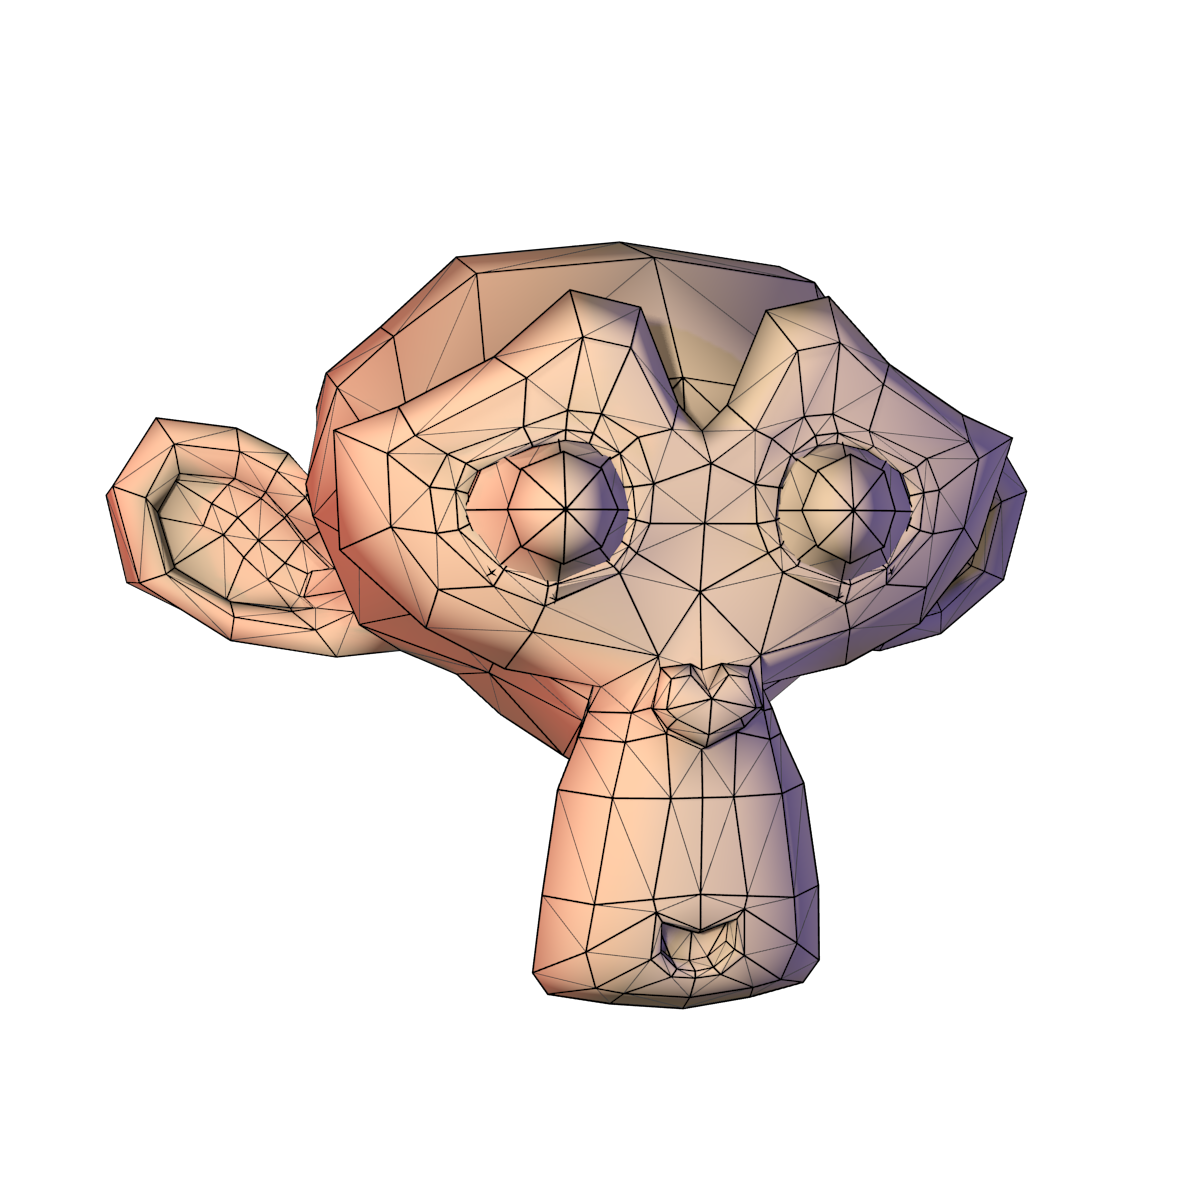
\includegraphics[width=0.25\textwidth]{./img/raw/coord-ruimtes/model_ruimte.png}};
    
    \node[inner sep=0pt] (img1) at (0.0\textwidth, -0.45\textwidth)
        {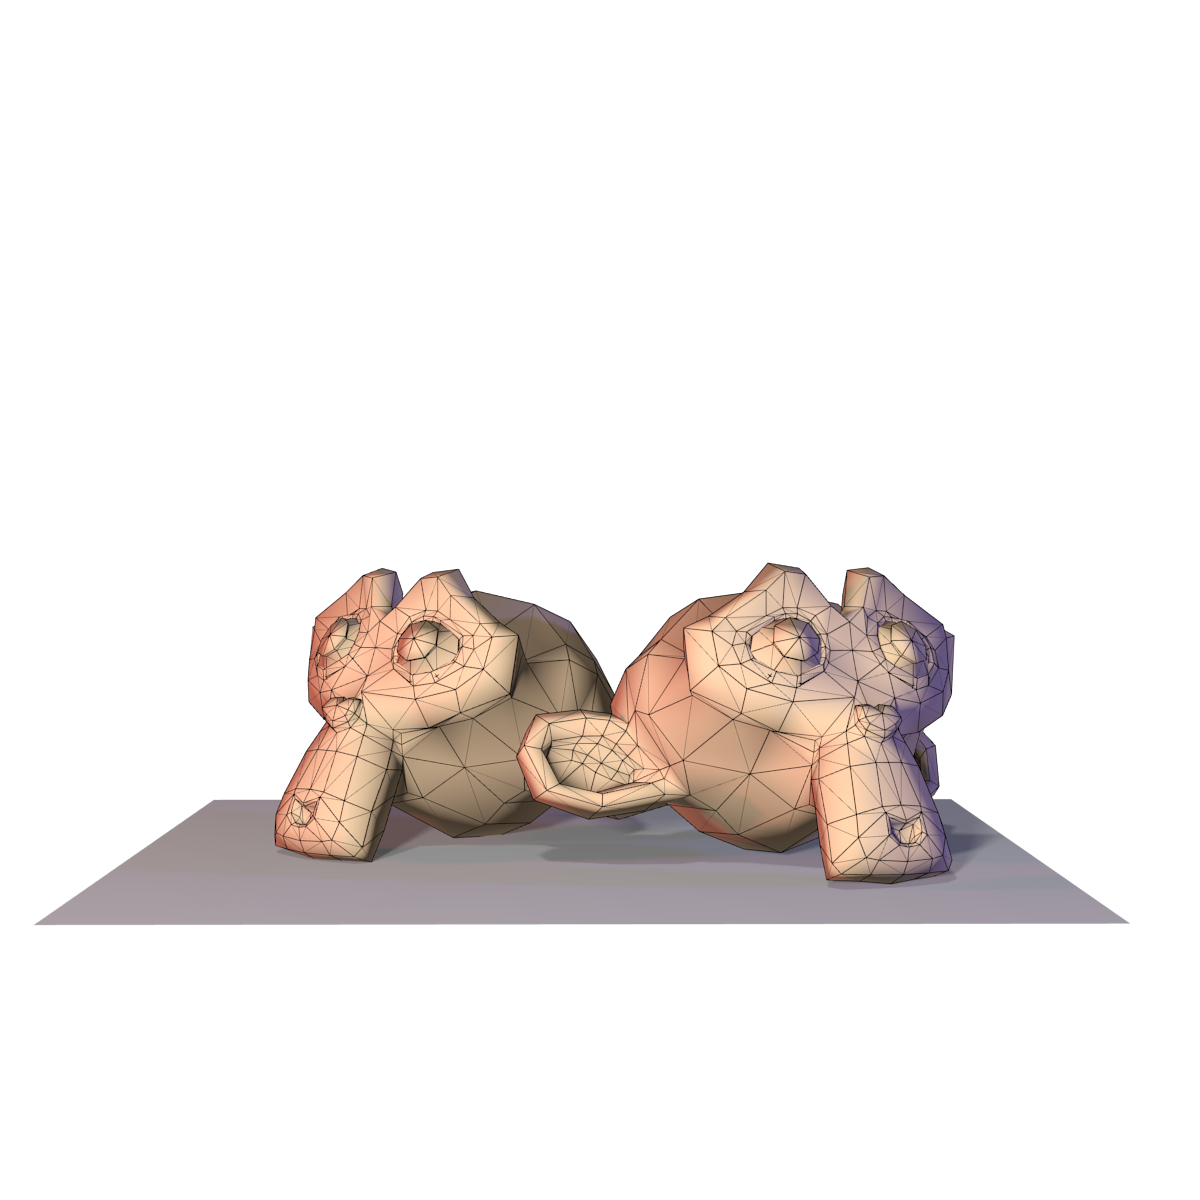
\includegraphics[width=0.6\textwidth]{./img/raw/coord-ruimtes/wereld_ruimte.png}};
    \node[inner sep=0pt] (img1) at (0.0\textwidth, -0.45\textwidth)
        {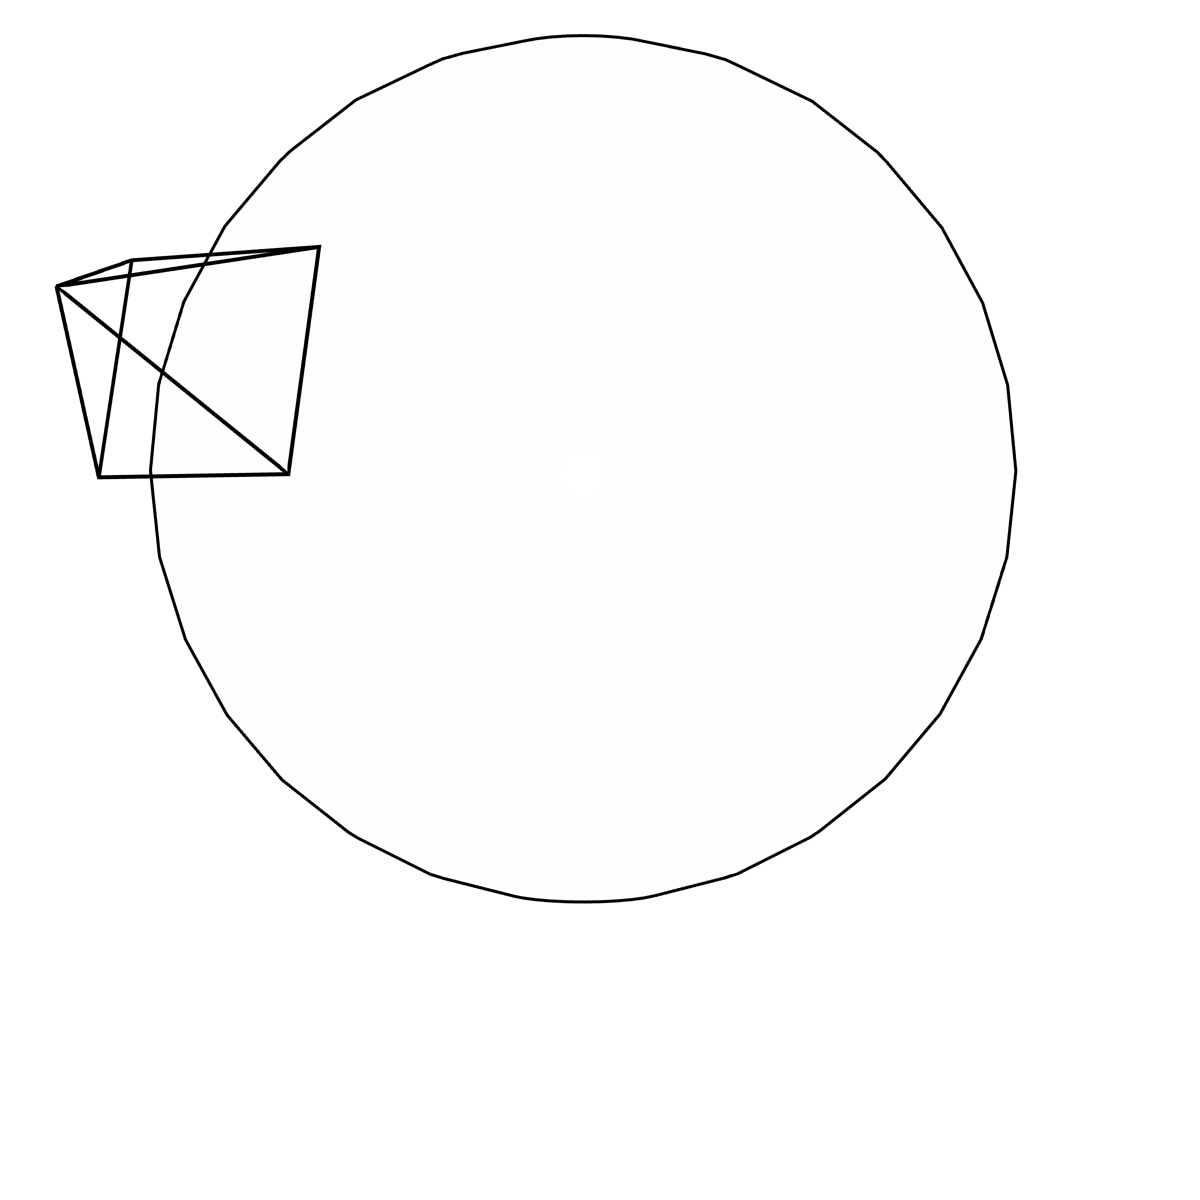
\includegraphics[width=0.6\textwidth]{./img/raw/coord-ruimtes/wereld_ruimte2.png}};
    
    \node[inner sep=0pt] (img1) at (0.0\textwidth, -1.05\textwidth)
        {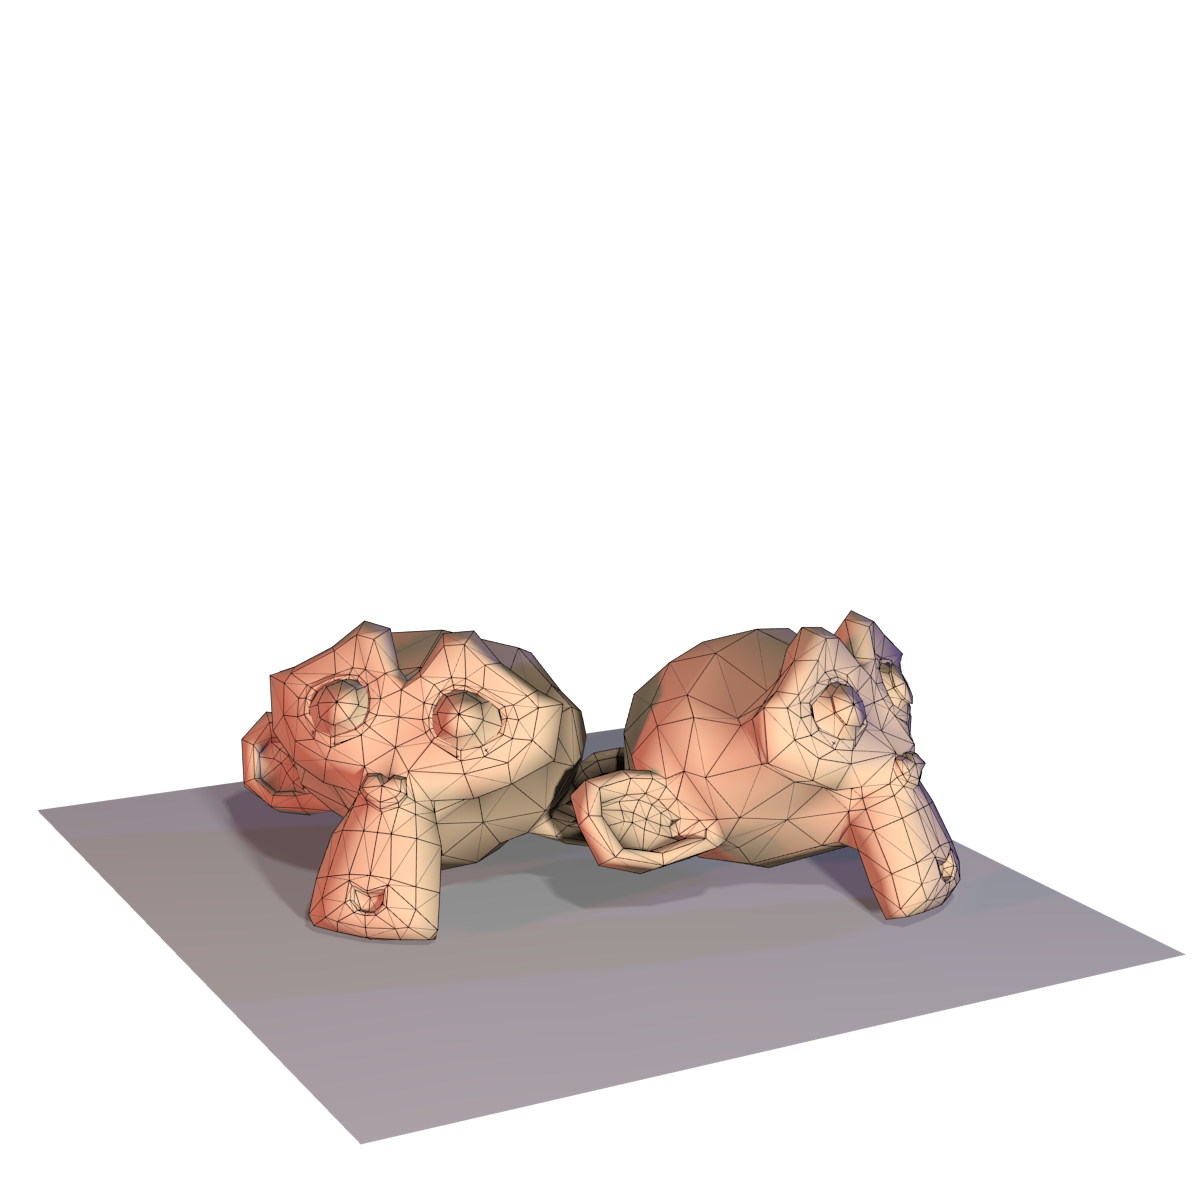
\includegraphics[width=0.6\textwidth]{./img/raw/coord-ruimtes/camera_ruimte.png}};
    \node[inner sep=0pt] (img1) at (0.0\textwidth, -1.05\textwidth)
      {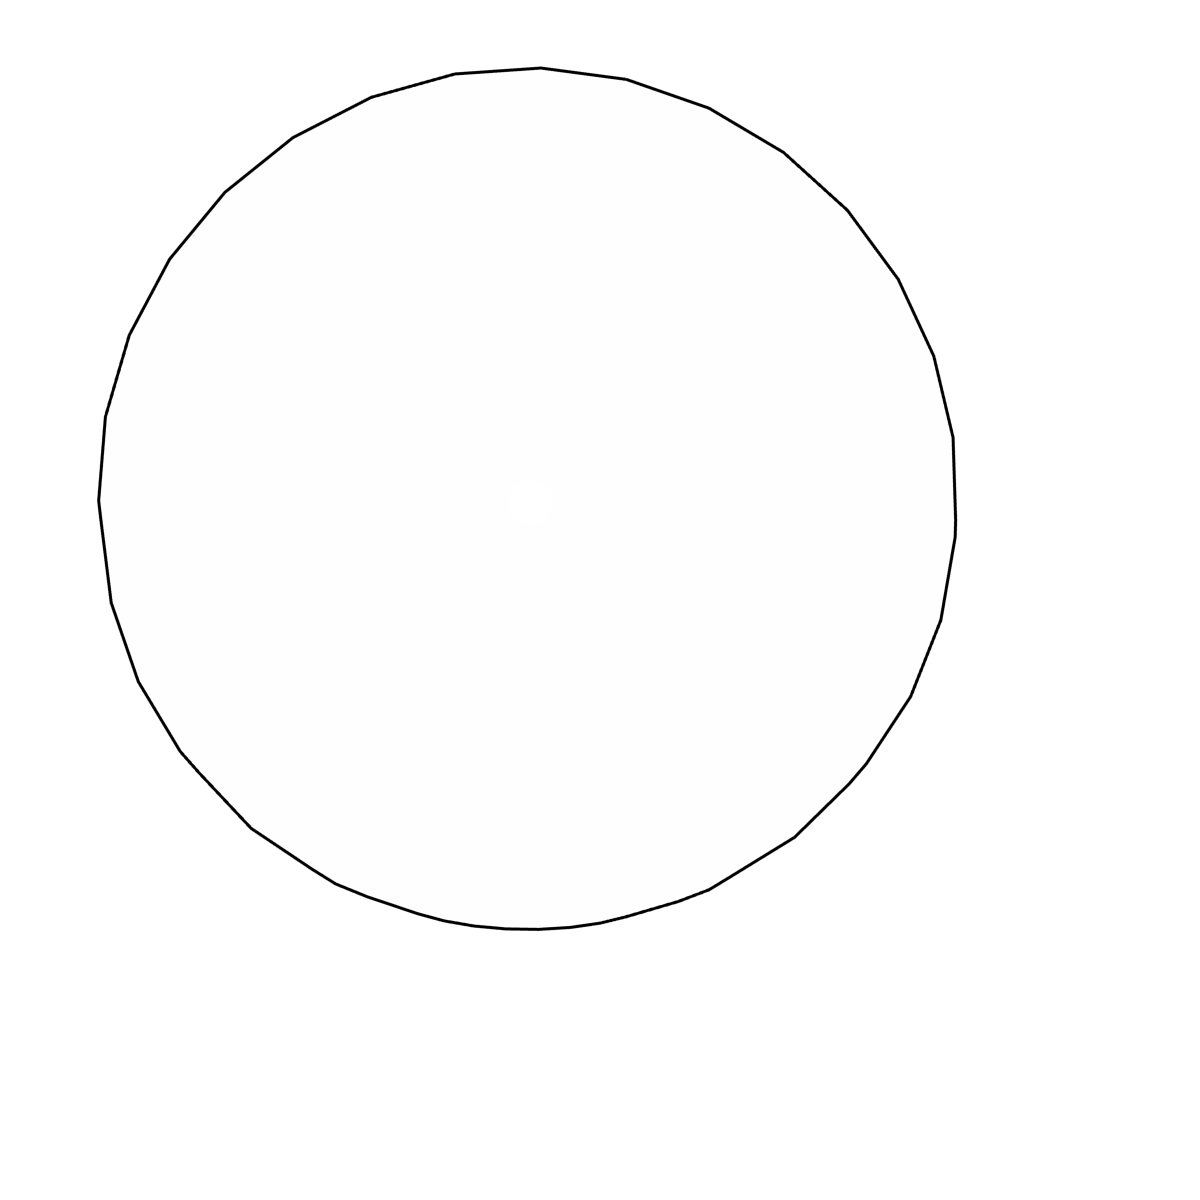
\includegraphics[width=0.6\textwidth]{./img/raw/coord-ruimtes/camera_ruimte2.png}};
    \node[inner sep=0pt] (img1) at (-0.125\textwidth, -0.0\textwidth)
        {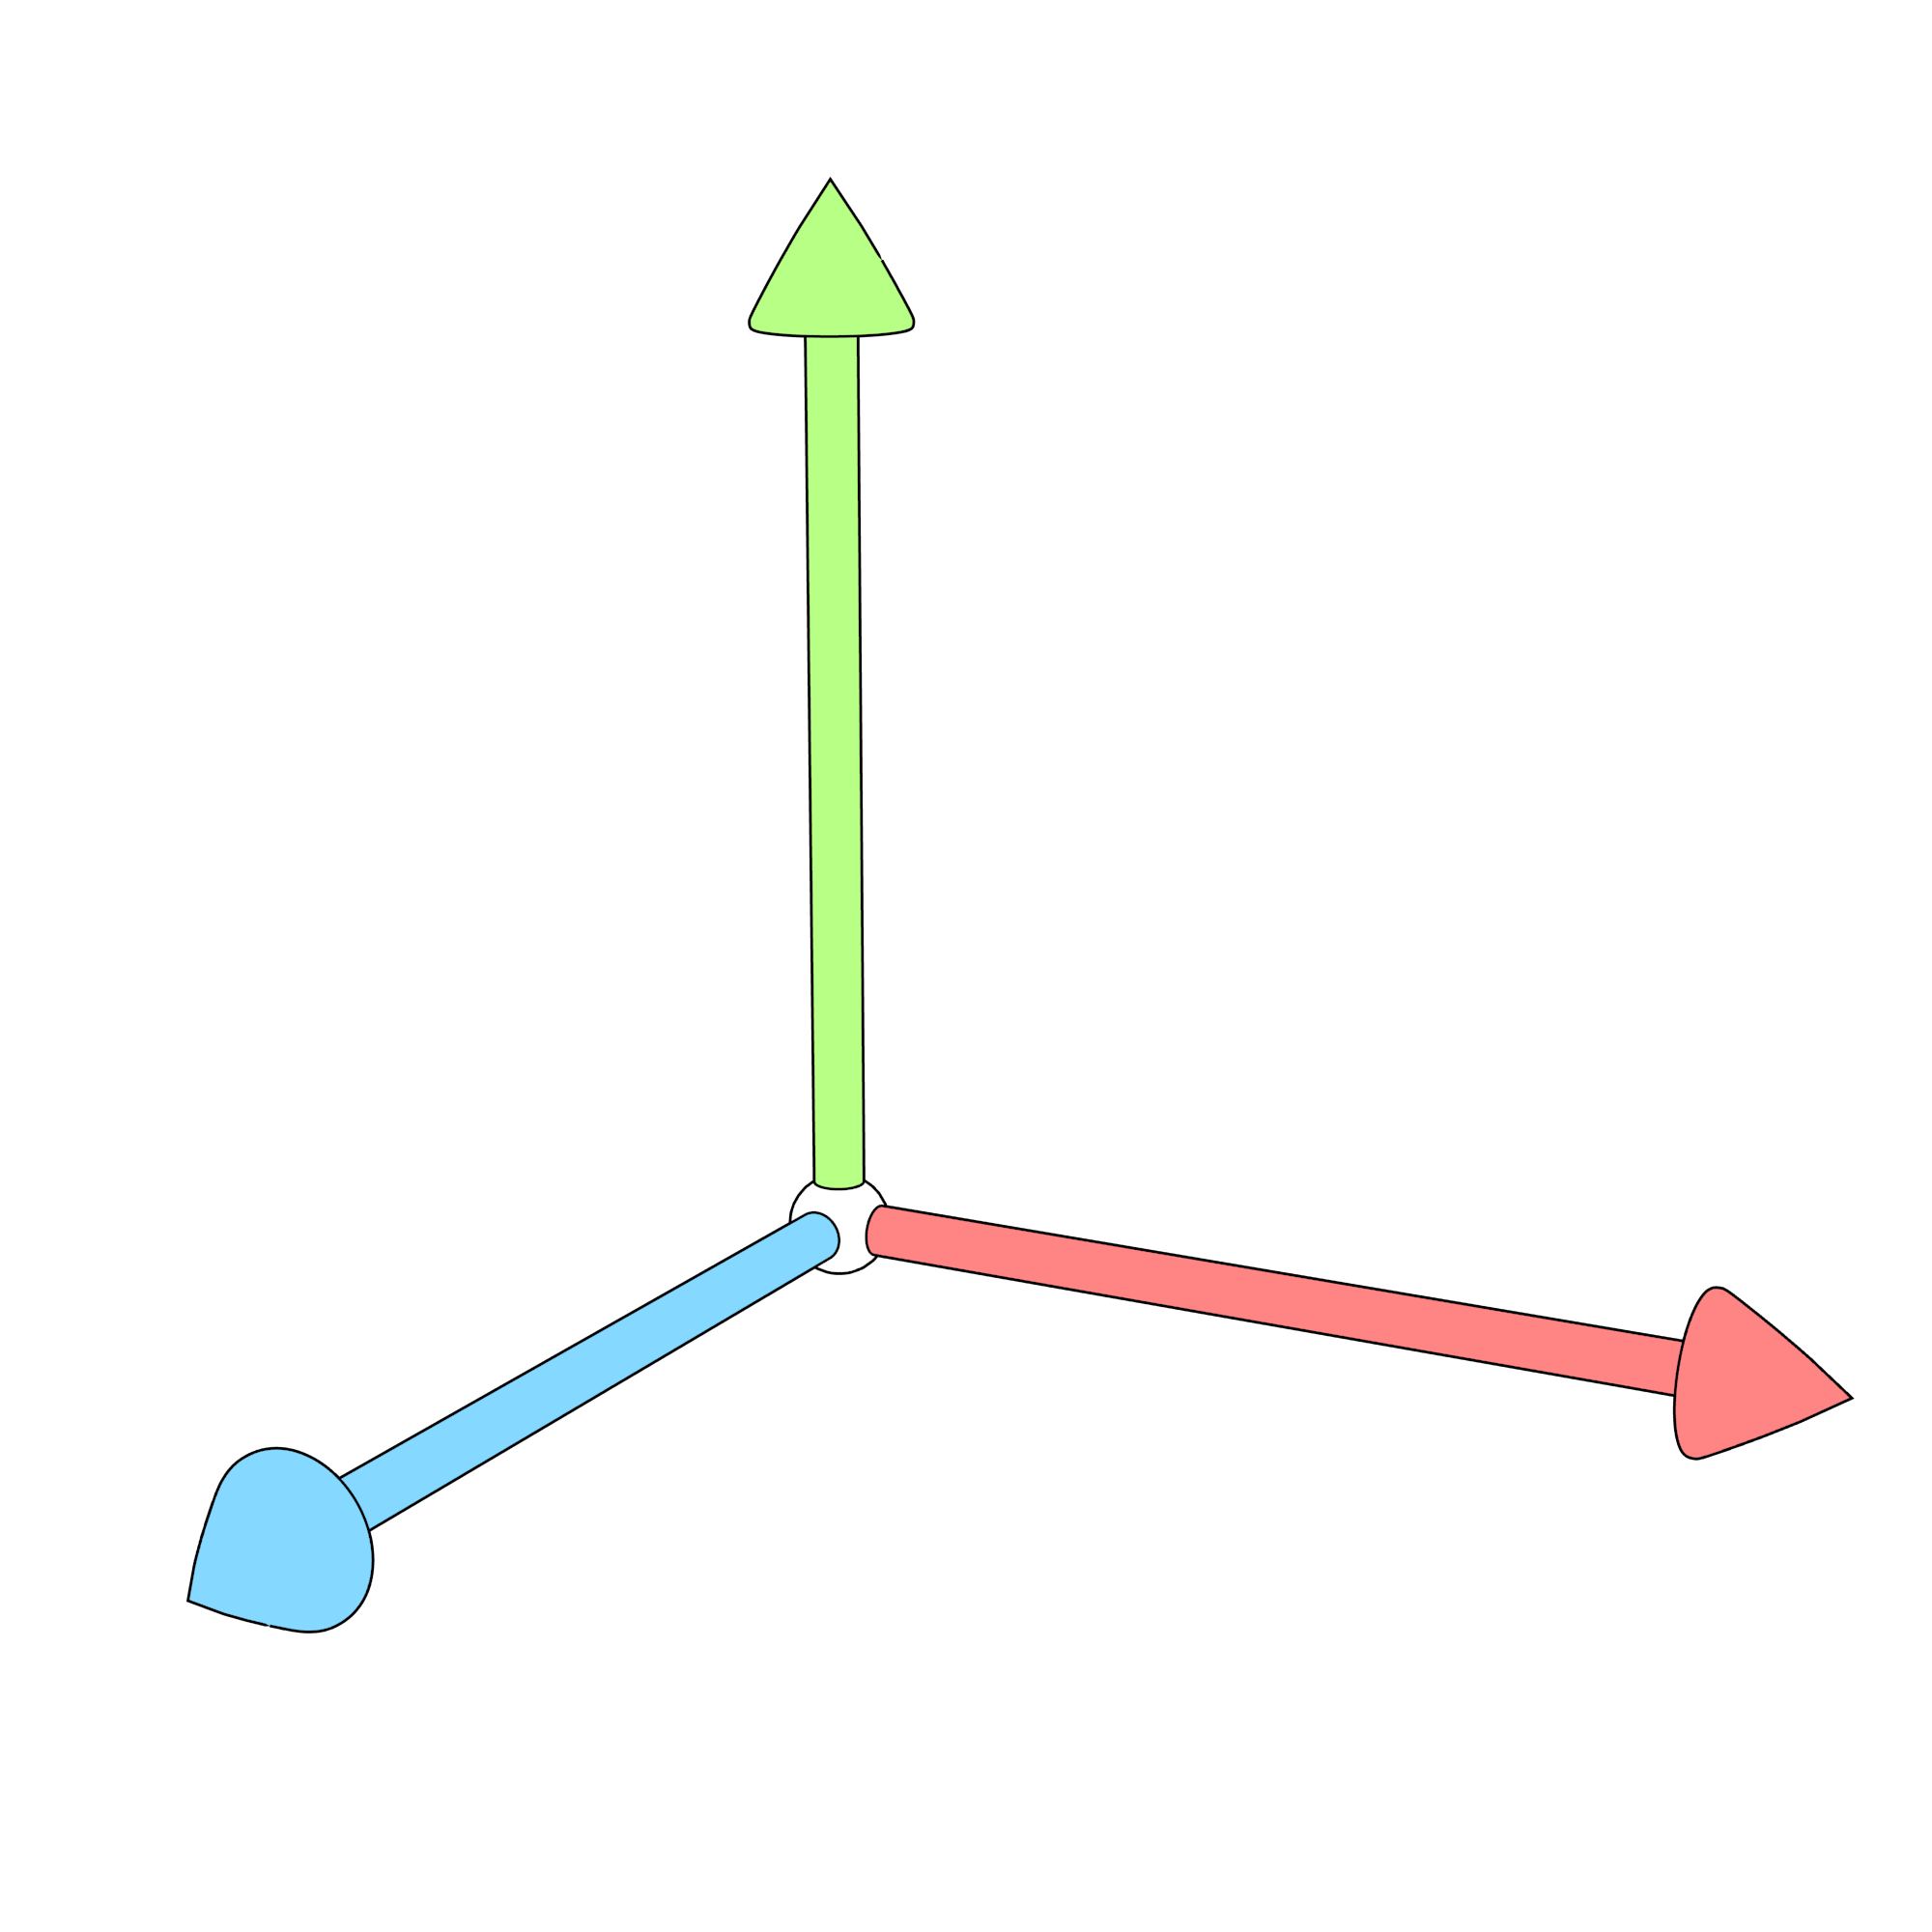
\includegraphics[width=0.125\textwidth]{./img/raw/coord-ruimtes/assen.png}};
    \node[inner sep=0pt] (img1) at (-0.25\textwidth, -0.525\textwidth)
        {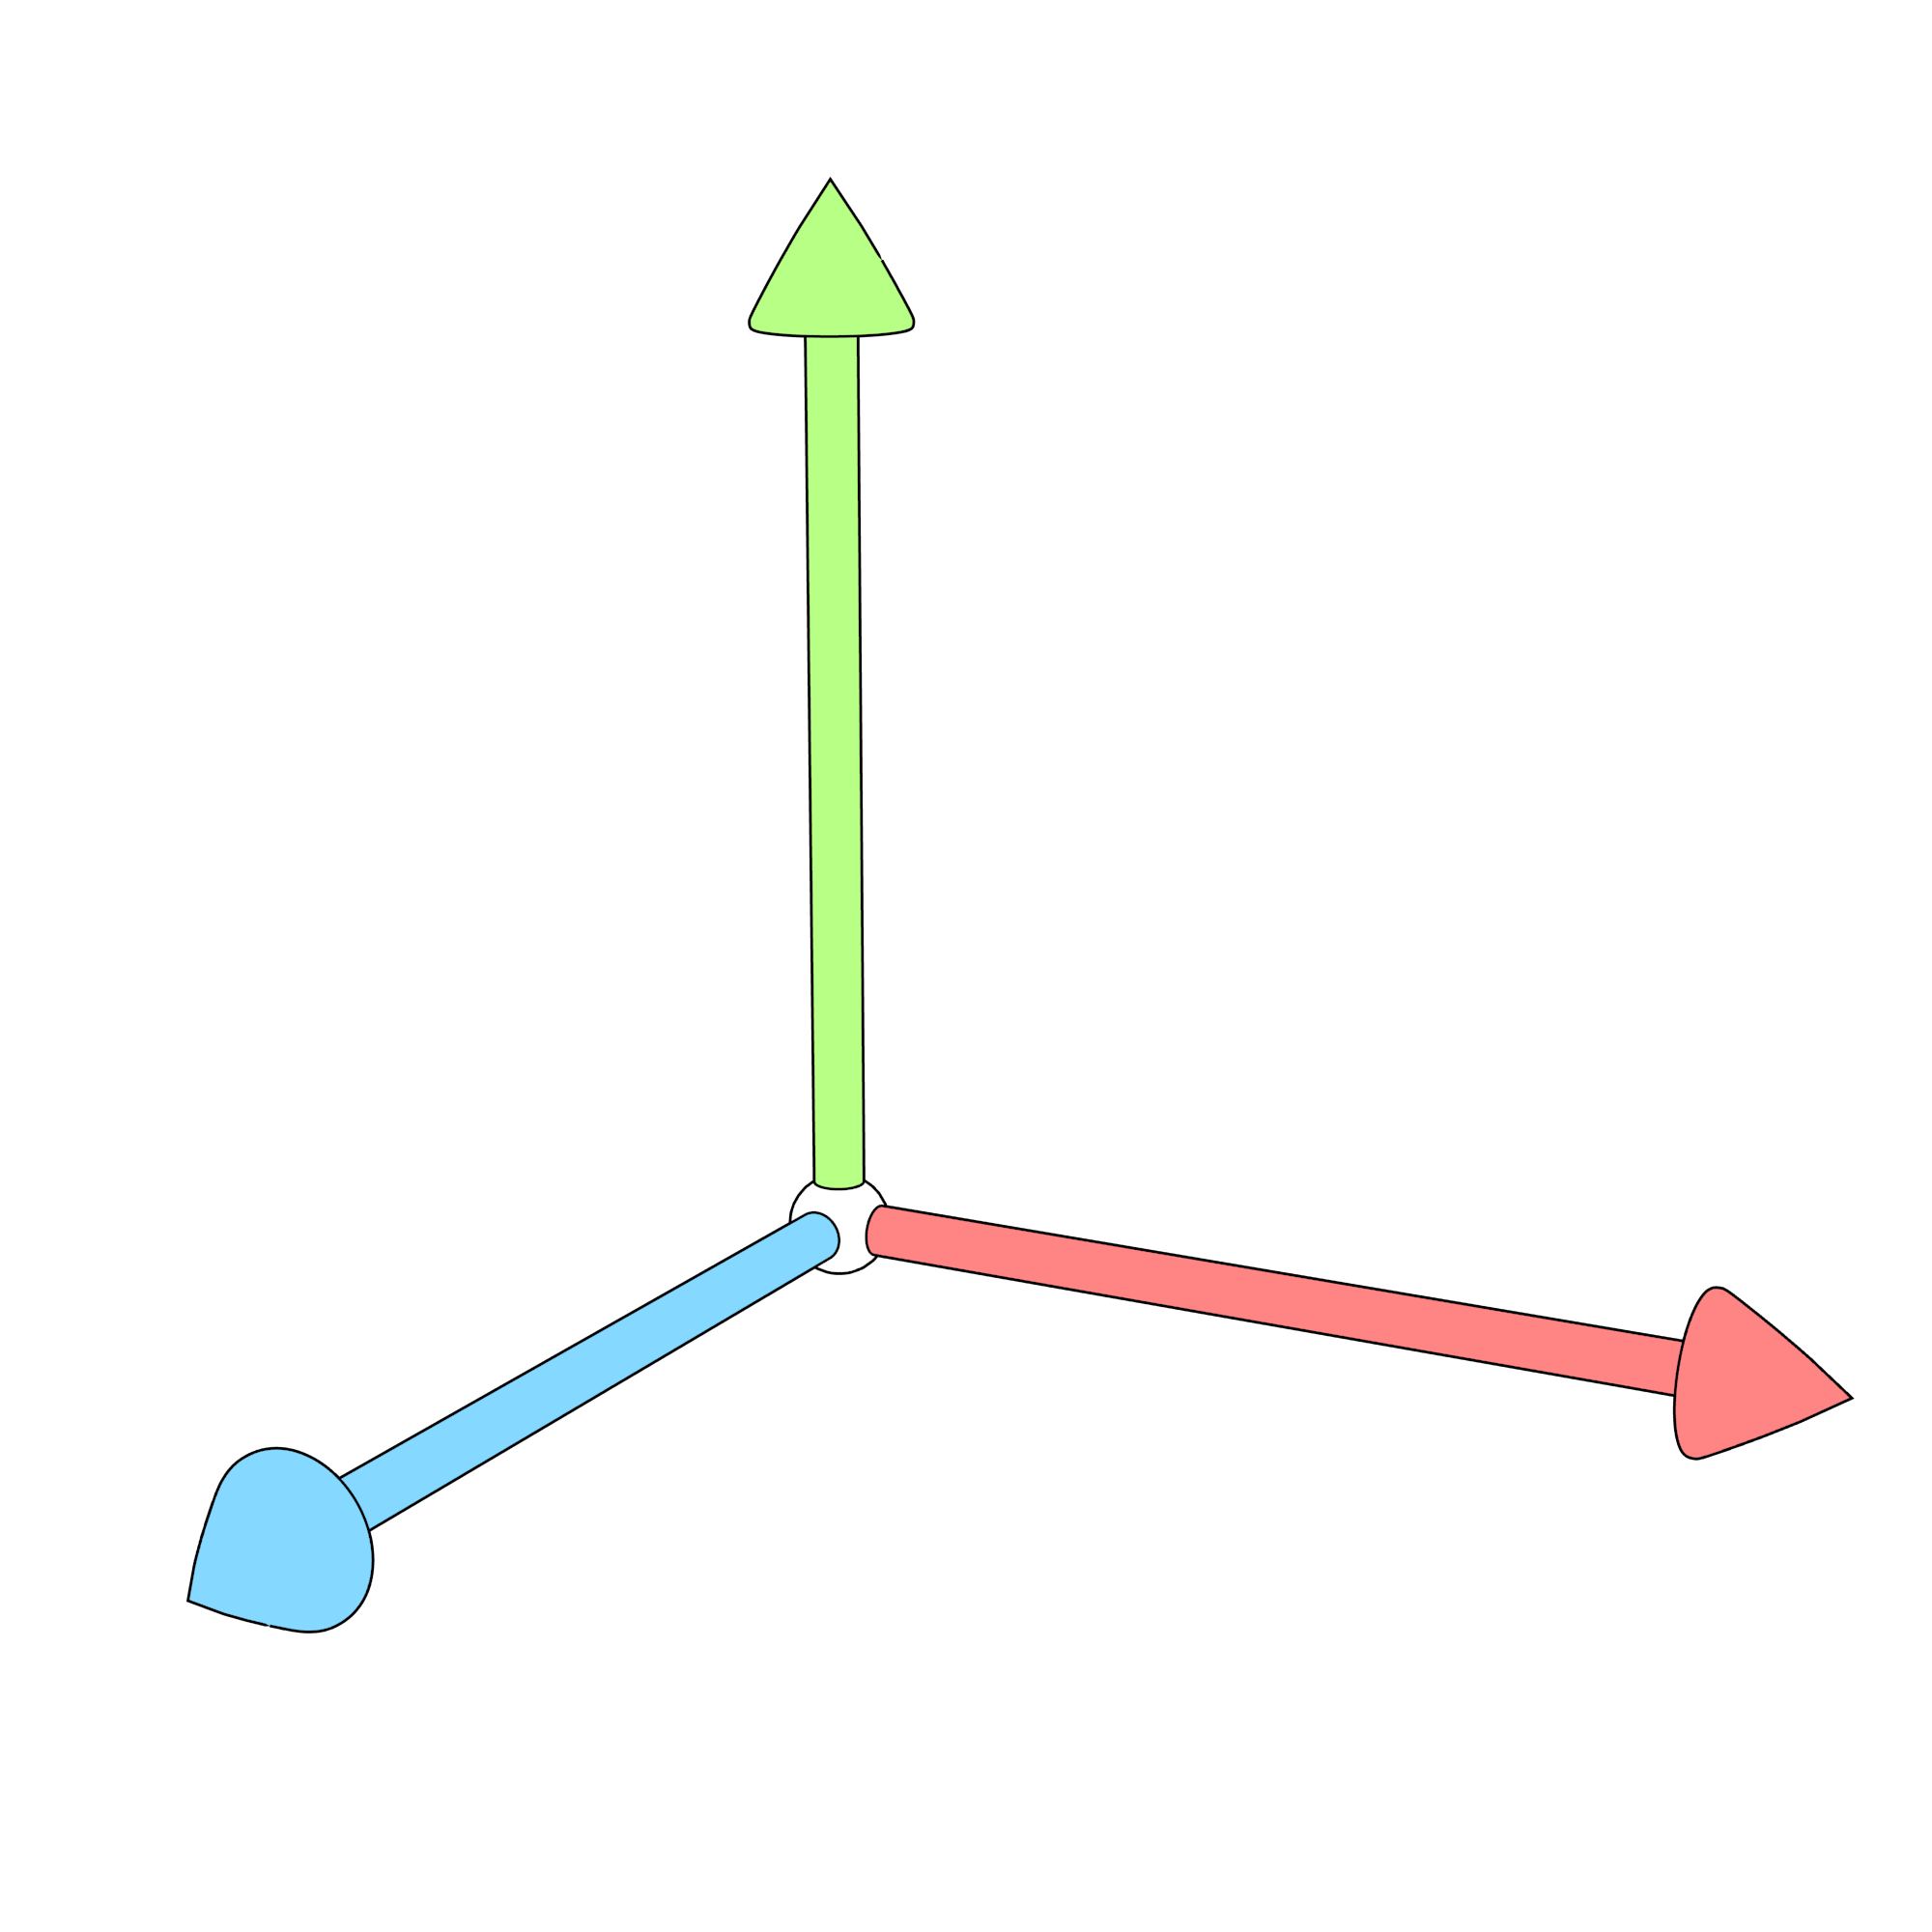
\includegraphics[width=0.125\textwidth]{./img/raw/coord-ruimtes/assen.png}};

    \draw[-stealth, thick] (-0.005\textwidth,-0.055\textwidth) -- (-0.005\textwidth,-0.15\textwidth);
    \draw[stealth-, thick] (-0.015\textwidth,-0.055\textwidth) -- (-0.015\textwidth,-0.15\textwidth);

    \draw[-stealth, thick] (-0.005\textwidth,-0.655\textwidth) -- (-0.005\textwidth,-0.75\textwidth);
    \draw[stealth-, thick] (-0.015\textwidth,-0.655\textwidth) -- (-0.015\textwidth,-0.75\textwidth);

    \node (l3) at (0.22\textwidth, -0.095\textwidth) {Object transformatiematrix};
    \node (l3) at (0.22\textwidth, -0.7\textwidth) {LookAt camera matrix};
  \end{tikzpicture}
  \caption{Verschillende Carthesische co\"ordinatenstelsels en bijbehorende transformaties.}
  \label{fig:coord-ruimtes}
\end{figure}
